\begin{frame}{ANNEXE}
\framesubtitle{Using permutations instead of pivots}
\begin{columns}[c]
\begin{column}{0.02\textwidth}
\end{column}
\begin{column}{0.45\textwidth}
\begin{center}
Using pivots
\includegraphics[width=\textwidth]{pivots_step}
\end{center}
\end{column}
\vline
\begin{column}{0.02\textwidth}
\end{column}
\begin{column}{0.45\textwidth}
\begin{center}
\visible<2>{Using permutations}
\includegraphics<2>[width=\textwidth]{permutations_step}
\end{center}
\end{column}
\end{columns}
\end{frame}

\begin{frame}{Update Problems}
\framesubtitle{Natural task flow of one swap in update}
\begin{center}
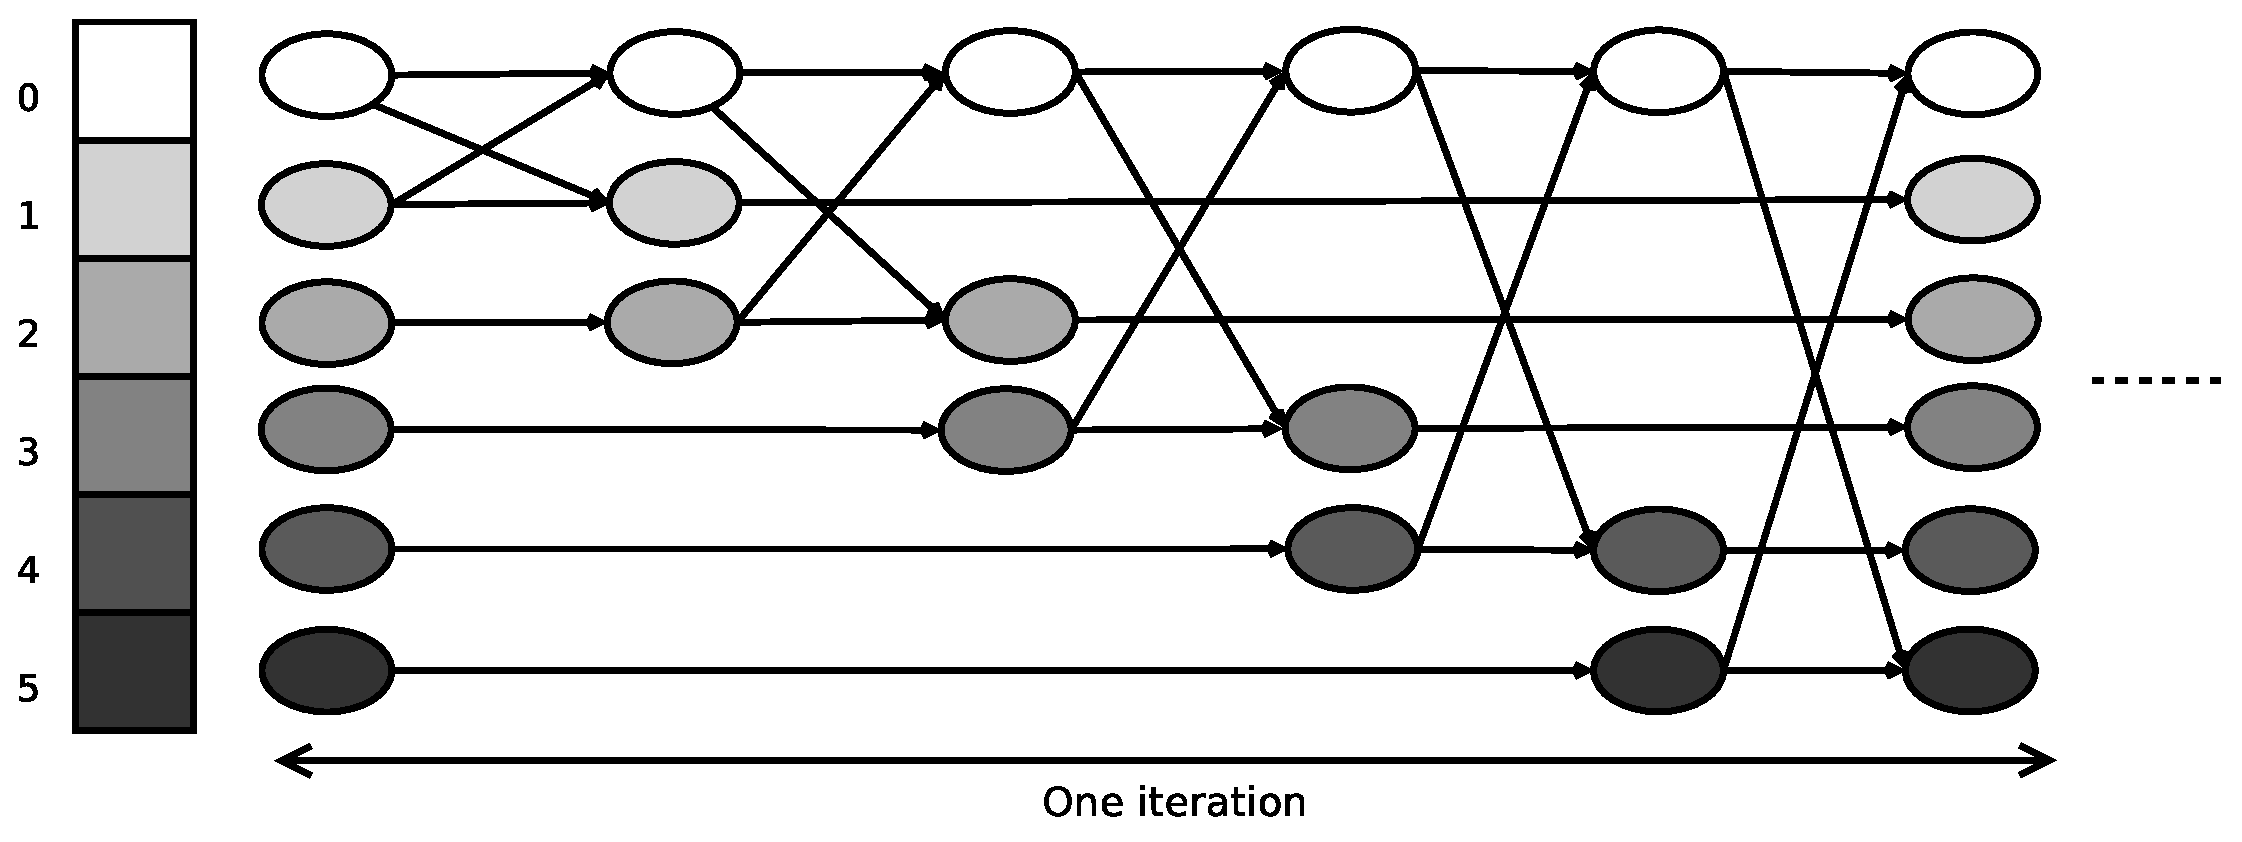
\includegraphics[width=0.6\textwidth]{natural_swap_tf_bw}
\end{center}
%\pause
%\begin{center}
%$\Rightarrow$ Huge number of synchronizations!
%\end{center}
%\pause
%\begin{exampleblock}{Optimizations:}
%Do all swaps in one single iteration by using permutations instead of pivots
%\end{exampleblock}{}
\end{frame}

\begin{frame}{Update Problems}
\framesubtitle{Optimized task flow of swaps of update for distributed architectures}
\begin{columns}
\begin{column}{.45\textwidth}
\begin{flushright}
\includegraphics<1,3>[scale=0.2]{swap_from}
\end{flushright}
\end{column}
\begin{column}{.50\textwidth}
\begin{flushleft}
\includegraphics<2,3>[scale=0.2]{swap_into}
\end{flushleft}
\end{column}
\end{columns}
\begin{center}
\includegraphics<4>[width=0.9\textwidth]{distributed_update_tf_bw}
\end{center}
\end{frame}

\begin{frame}{Update Problems}
\framesubtitle{Optimized task flow of swaps of update  for hierarchical architectures}
\begin{center}
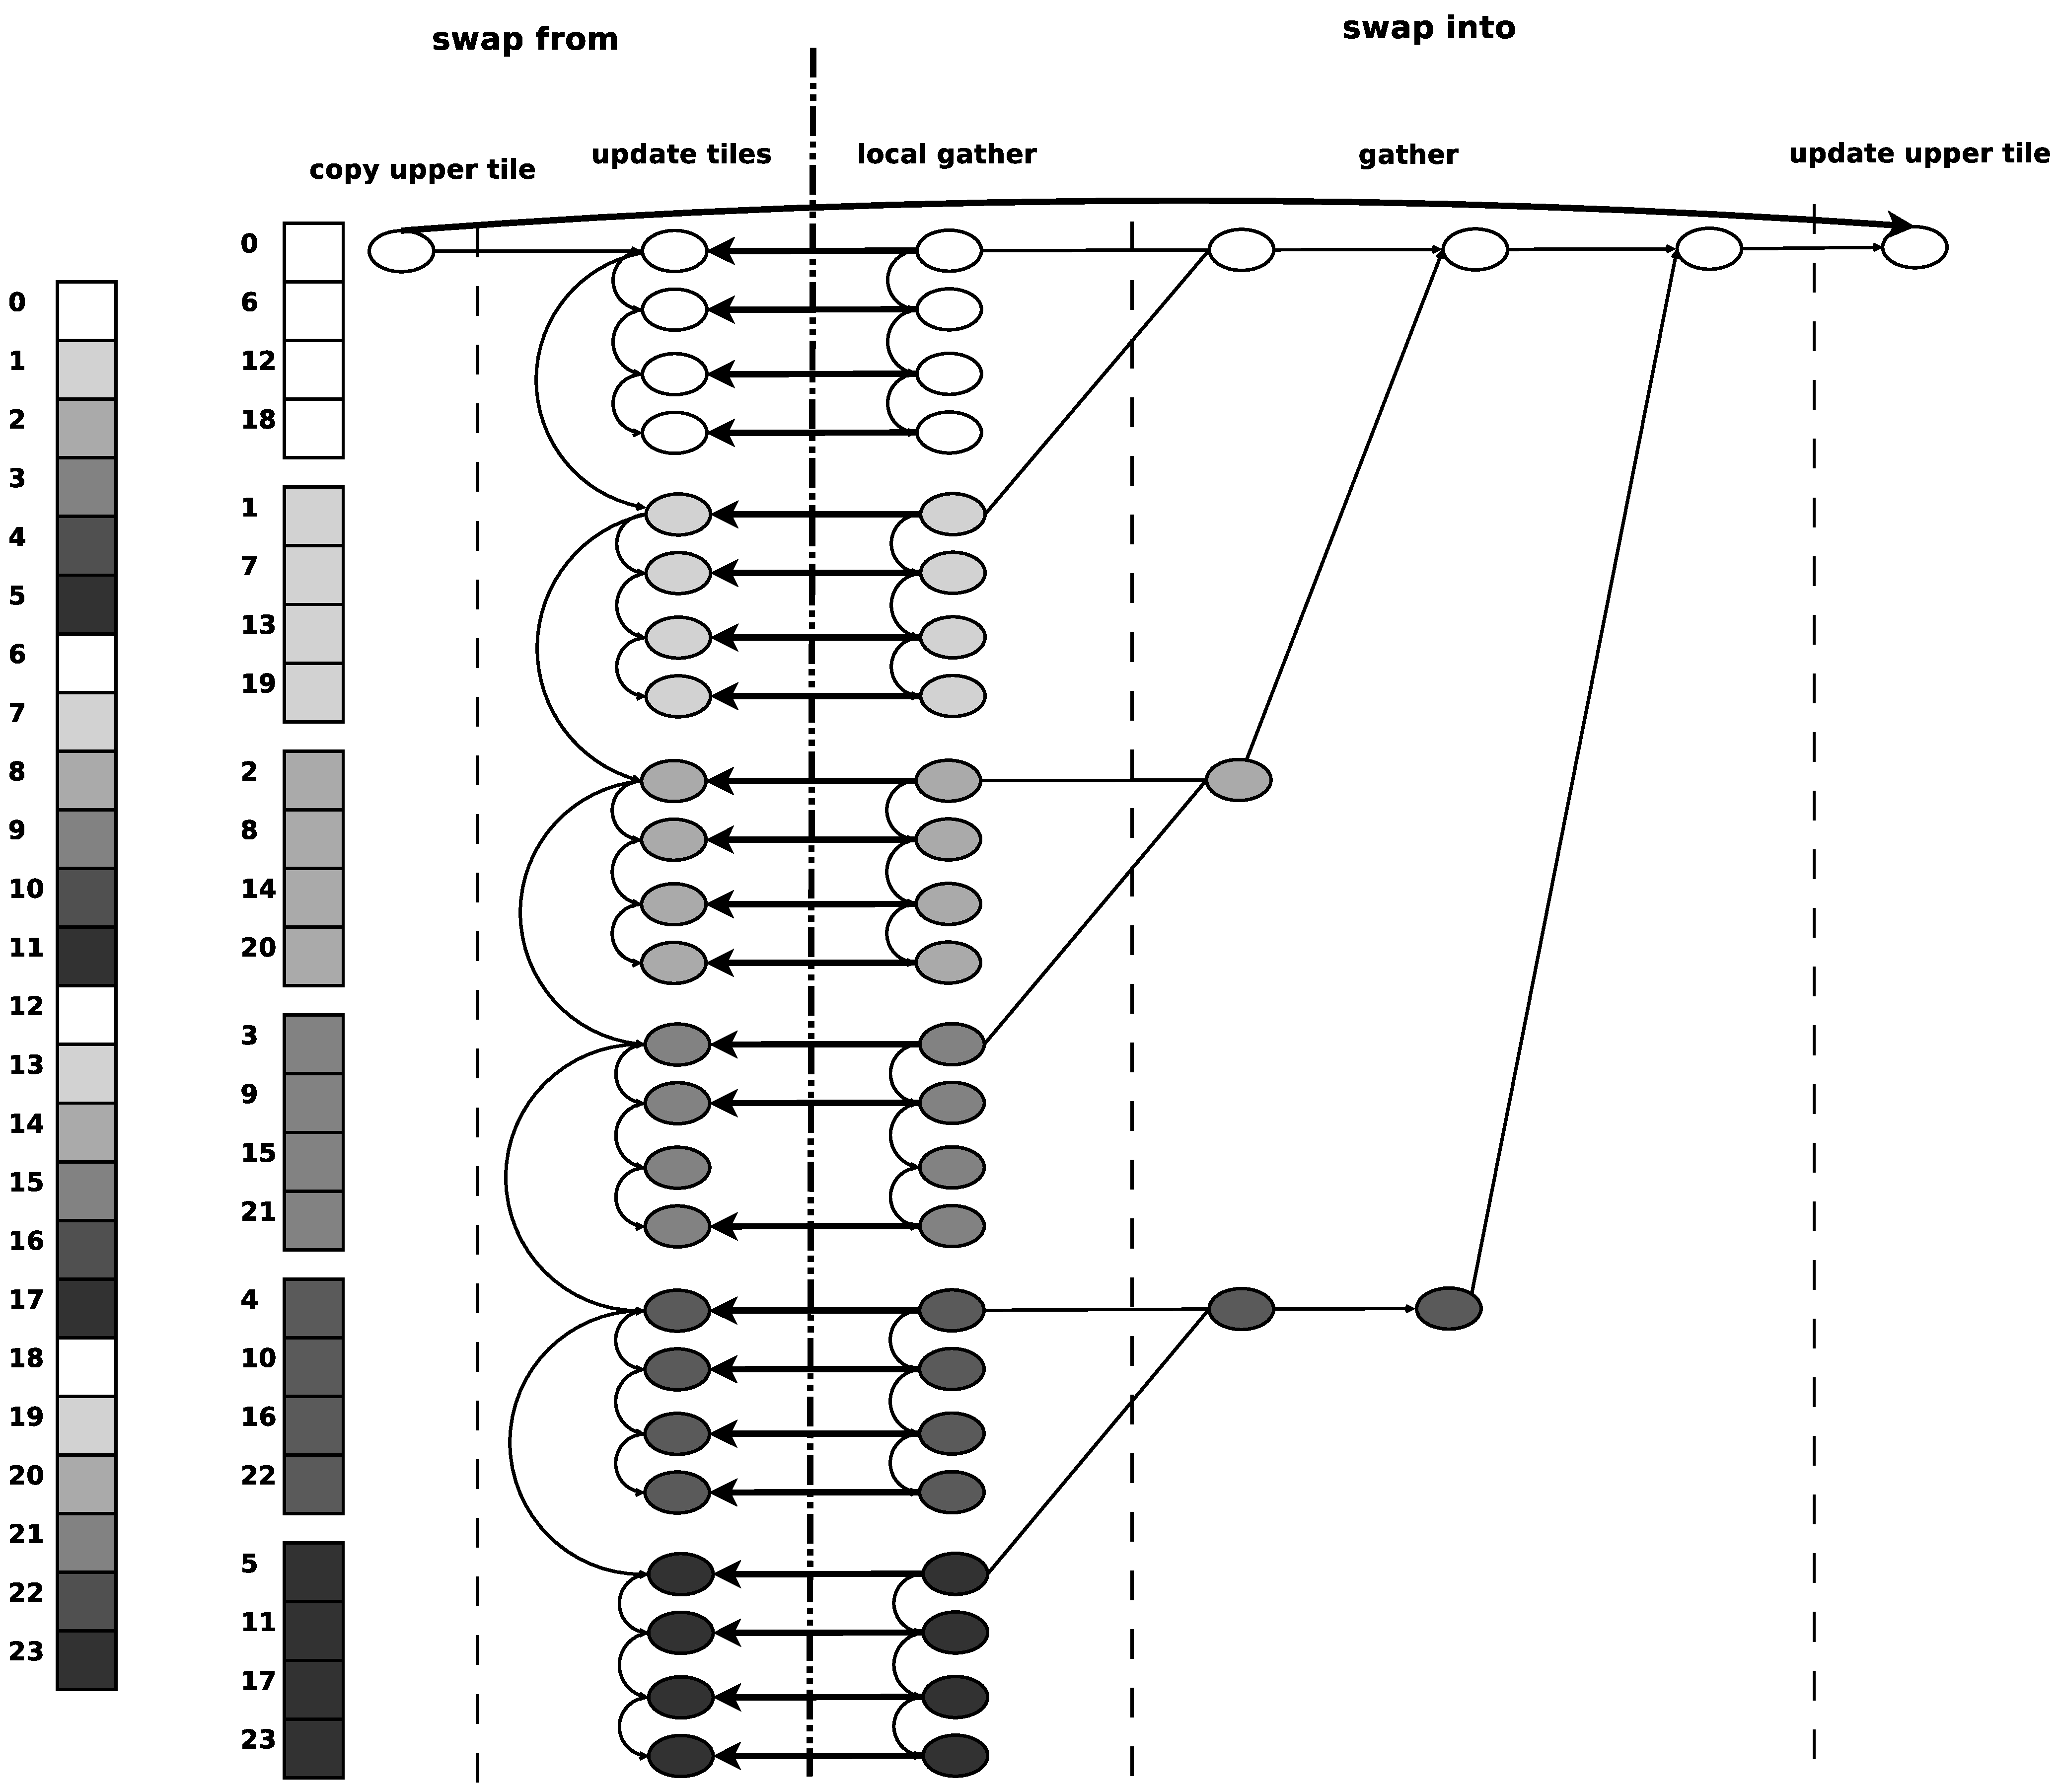
\includegraphics[width=0.65\textwidth]{update_tf_bw}
\end{center}
\end{frame}
